\chapter{The \textsl{Sound Pattern of English} and its aftermath}
\label{ch.spe}

There are surely few years that are so clearly marked as watersheds in
the history of phonology as 1968. In that year, \citeauthor{spe}
published their long-awaited work \textsl{The Sound Pattern of
  English} (referred to as \textsl{\isi{SPE}} below), by far the most
comprehensive presentation and exemplification of the theory of
generative phonology to appear up to that point (or since, for that
matter). The manuscript had circulated in various versions for several
years before, but its final appearance made the theory available for
much more general analysis and criticism than had hitherto been
possible. Although earlier publications had described the theory, as
discussed in the previous chapter, 1968 was the year in which
generative phonology was finally in complete enough form for
substantive scrutiny.

The publication of \textsl{\isi{SPE}} also had another, symbolic
importance. It marked the end of an era in which the major works of
generative linguistics (in syntax as well as in phonology) were
circulated primarily in \emph{samizdat'} form among a small circle of
insiders, with those not on the necessary mailing lists confined to
secondhand reports and rumors for their information on the shape of
theoretical developments.\footnote{Although
  \citet[ch. 5]{newmeyer22:ailt} argues that the ‘underground press’
  played a much smaller role than is commonly believed in the early
  days of \isi{generative grammar}, and that all of the leading lights of
  this period, and their students, were prolific publishers.} Overt,
formal publication of a reasonably definitive description of the
principles of the theory made it much more a matter of public
property, and enfranchised a much broader audience of potential
contributors and critics. And, as this wider accessibility was
broadening their audience, generative linguists were increasingly
turning to the {regular} avenues of formal book and journal publication
(in some instances, creating their own, such as \textsl{Linguistic
  Inquiry}) rather than to their duplicating machines. The number of
significant papers whose reference sections were essentially confined
to unpublished work plummeted.

If 1968 was the year in which generative phonology was substantiated
and legitimized, it was also the year from which the reaction against
the theory must be dated. Before, objection had come largely from
those wishing to maintain some form of American (or European)
structuralist view; but by the time of the appearance of \textsl{\isi{SPE}},
this had ceased to be an issue for all but a few. From then on, the
objections that were raised came from within the general perspective
on language that {\Chomsky} and {\Halle} had established, and sought to
question generative theory on its own terms. Since much of this
discussion continued for many years, it would be ridiculous to attempt
a definitive summary of it and its results; the present chapter aims
simply to characterize the most important attempts to revise or
replace the theory of \textsl{\isi{SPE}}.


\section{The nature of the \textsl{SPE} program}

A useful perspective on the issues involved in generative phonology
can be ob\-tained from a consideration of parallels between the evolution
of phonological theory and that of the foundations of
\isi{mathematics}.\footnote{The comparison here between the histories of
  phonology and of \isi{mathematics} is drawn from the discussion in
  \protect\citealt{sra80:copenhagen}.} Let us recall that the nature
of a phonological theory as expressed in \textsl{\isi{SPE}} centers on an
explicit formal notation for phonological description. In combination
with an evaluation function for grammars defined over this notation,
this would constitute a comprehensive axiomatization of the subject
matter of phonology, in the sense that all problems connected with the
discovery of correct (or `descriptively adequate') accounts of sound
structure would thereby be reduced to the mechanical manipulation of
expressions in a fully explicit \isi{notational system}. Of course,
\citet{spe} do not claim to have accomplished this goal, but it is
nonetheless the program of the theory. The successes achieved within
the framework of `classical' generative phonology were seen as
confirmation of the plausibility of such an axiomatization.

In this respect, the program of \textsl{\isi{SPE}} is strikingly similar to
that of another fundamental work of twentieth-century thought,
\posscitet{whitehead.russell10-13:principia} \textsl{Principia
  Mathematica} (cited as \textsl{PM} below). That work enunciated and
developed a goal of reducing all of the intellectual content of
\isi{mathematics} to the formal manipulation of expressions in a logistic
system by means of fully explicit rules. While the calculus of formal
logic in which \textsl{PM} proposed to express mathematical
propositions is of course quite unlike the descriptive apparatus
envisaged by \textsl{\isi{SPE}} for phonological expressions, and {\Chomsky}
and {\Halle} never refer to
\citeauthor{whitehead.russell10-13:principia}, the intent of
expressing all of the content of their respective fields in terms
subject to formal manipulation by means of well-established rules is
common to the two works.

\textsl{PM}'s account of the foundations of \isi{mathematics} was initially
greeted with enthusiasm, since it promised to give a full
reconstruction of the traditional notion that the truth of
mathematical propositions derives from logic alone, and not from
contingent facts about the world. This enthusiasm soon gave way to
dissatisfaction, however, as it became apparent that there were
fundamental obstacles to the logicist program. In particular, the
theory in its {basic form} was seen to give rise to a number of the
paradoxes which had long been troublesomely familiar to
mathematicians, such as various forms of the problem of the barber who
shaves everyone who does not shave himself, and other apparent
self-contradictions. In order to remedy this difficulty, Russell\ia{Russell, Bertrand} had
proposed what is known as the theory of `types': roughly speaking, a
restriction on the kinds of classes that can be referred to in any
given expression.

Unfortunately, the \isi{theory of types} itself had undesirable
consequences: it rendered many of the basic propositions of number
theory unstatable or meaningless. It was thus necessary, in the full
system of the \textsl{PM}, to appeal to an `axiom of infinity' and an
`axiom of reducibility', whose plausibility and intuitive appeal are
vastly less than that of the rest of the logical system. Since the
\isi{theory of types} seemed unavoidable in the context of the logic of the
\textsl{PM}, and since it seemed to lead to such counterintuitive
emendations of the system, the logicist program for the foundations of
\isi{mathematics} was gradually abandoned.

Partially in response to the perceived failure of this approach, other
views of the foundations of \isi{mathematics} were developed on other
assumptions. Among the most important of these alternatives was that
presented by \name{L. E. J.}{Brouwer} and others under the title of
`\isi{intuitionism}'. A primary tenet of this school is the rejection of all
expressions purporting to refer to objects that cannot in fact be
fully constructed. In particular, expressions that refer to explicitly
infinite sets are disallowed, since while one can give directions for
enlarging the extension of a set without limit, it is obviously not
possible to complete the enumeration of such an object. This move has
the immediate consequence that the paradoxes which arise within
Russell\ia{Russell, Bertrand}'s system are avoided, since the problematic classes turn out
to be impossible to construct within the limits of an intuitionist
logic.

Intuitionists have attempted to reconstruct as much as possible of the
subject matter of \isi{mathematics}, while adhering to these strict
limitations on the invocation of explicitly infinite classes. In many
cases it has proved possible to reformulate classical results in such
a way that their essential content can still be derived in these
terms. In other areas, however, this cannot be done, and the
intuitionists are then led to conclude that these parts of \isi{mathematics}
(including much of traditional analysis) are in fact meaningless: a
somewhat controversial result.

In the course of developing the intuitionist program, its
practitioners have clearly revealed much about the conceptual basis of
mathematical propositions. This program does not really lead to
independent advances, however, since its goals are in fact much more
conservative ones, and it provides the basis for the development of
only a limited portion of mathematical work. Relatively few working
mathematicians seem willing to accept the limitations on their subject
matter imposed by the premises of intuitionist logic. Although it can
be said to have shed light on a (proper) subset of the field,
\isi{intuitionism} cannot be said to have provided a satisfactory
replacement for the traditional objects of study and modes of
inference in \isi{mathematics} as a whole.

\begin{wrapfigure}{l}{.45\textwidth}
  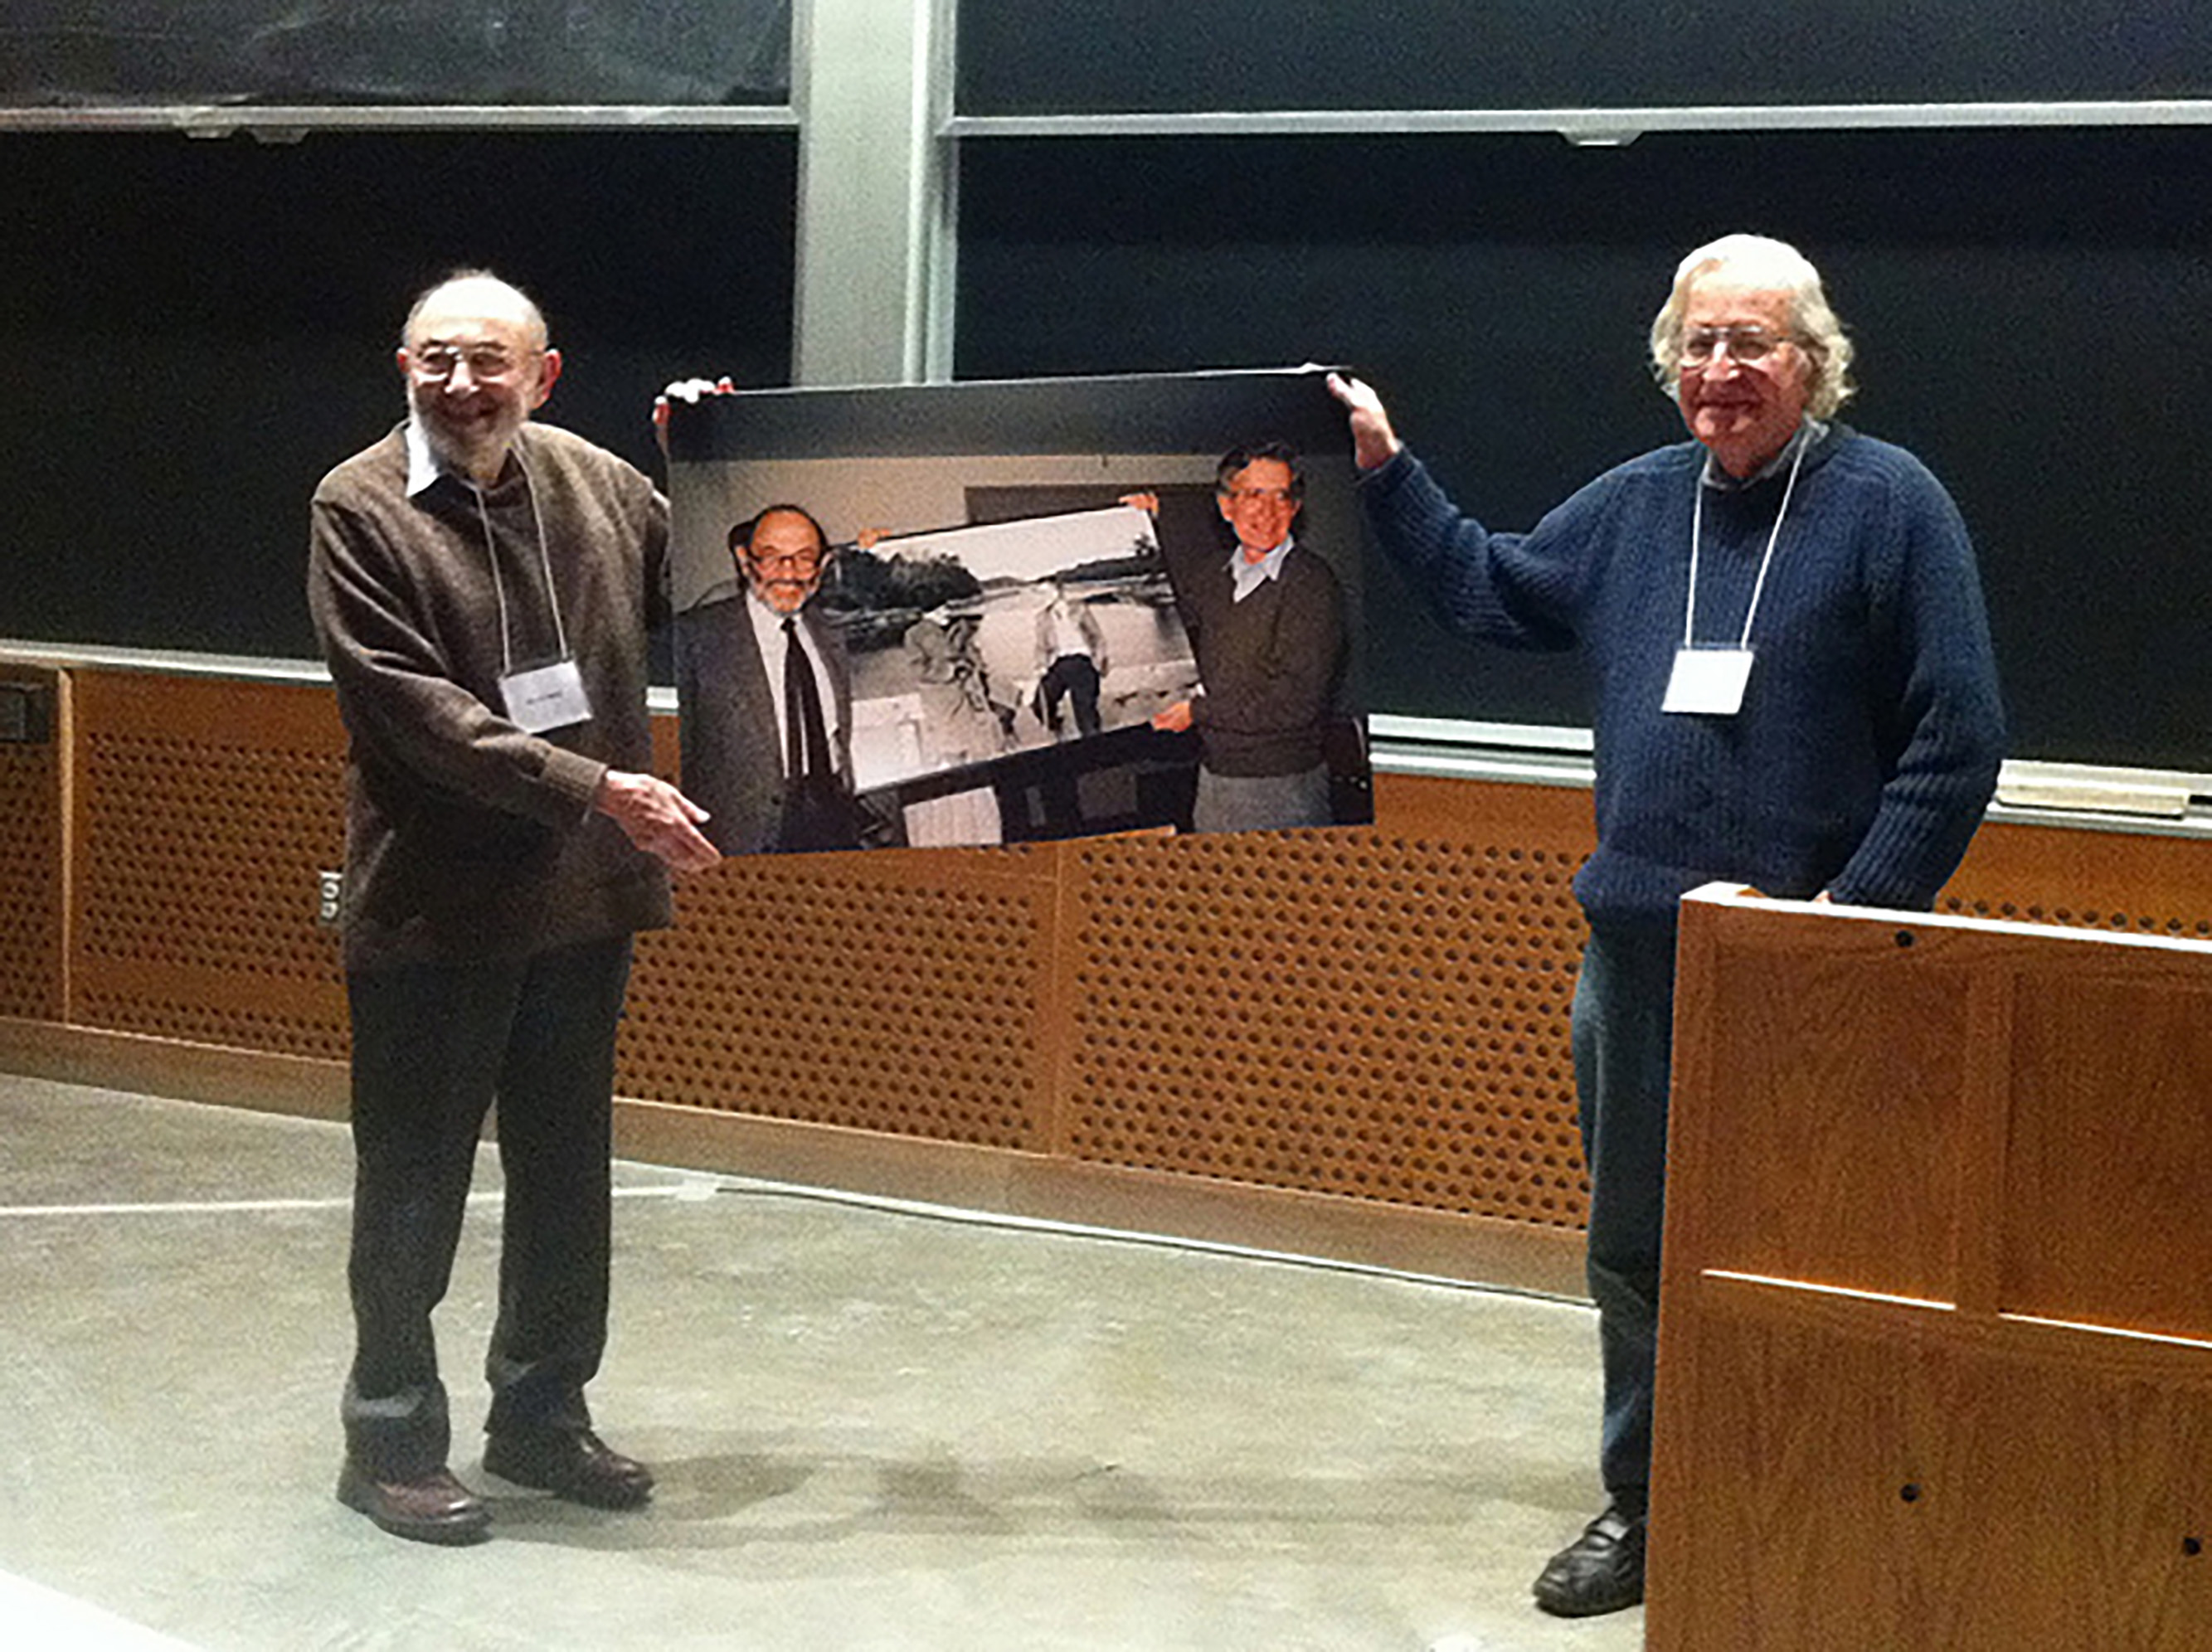
\includegraphics[width=.9\textwidth]{figures/morrisnoam50.jpg}
  \caption{Morris Halle and Noam Chomsky (2011 (1988 (1953)))}
  \label{fig:ch.spe.morrisnoam50}
\end{wrapfigure}
This history, though tangential to the history of phonology, is
rehearsed here because it provides an instructive parallel with the
development of phonological discussion in the years immediately after
the publication of \textsl{\isi{SPE}}. The substantive similarities between
the programs of \textsl{\isi{SPE}} and \textsl{PM} have already been pointed
out. We will suggest below that the phonetic \isi{arbitrariness} which was
immediately pointed out as a problem with the \textsl{\isi{SPE}} system
constituted an Achilles' heel similar to that of the classical
antinomies within the framework of \textsl{PM}; and that the theory of
`\isi{markedness}', which was proposed to remedy this defect, was as
inadequate a band-aid for phonology as the \isi{theory of types} was for the
mathematical logic of \textsl{PM}. Further, in attempting to deal with
these problems in more radical ways, some linguists have taken a line
quite comparable to that of the intuitionists in \isi{mathematics}—with
comparably limited success.

\section{The problem of phonetic content within the \textsl{{SPE}} theory}

The first line of attack on the \textsl{\isi{SPE}} program from within the
assumptions of \isi{generative grammar} is found in the final chapter of the
book itself. There it is observed that the purely formal calculus to
which phonological expressions are supposed to be reduced is
absolutely neutral as to the substantive content of the
\isi{representations} and rules appearing in particular descriptions. The
notation, that is, provides a vocabulary in the form of a set of
features and a formalism for rules; but within this vocabulary all
expressions are essentially homogeneous with respect to the formal
measure of evaluation which is intended to reconstruct the linguistic
significance of generalizations embodied in particular descriptions.

Central to the formal calculation of this measure is the set of
\isi{notational conventions}: these are intended to capture the extent to
which certain sets of rules in fact embody a unitary generalization,
and they do so on the basis of a purely formal manipulation of the
expressions representing the component rules. Thus, two rules are
collapsible by the parentheses notation exactly in the case where the
second can be obtained from the first by the omission of a single
contiguous sub-string. Schematically, the rules `A$\rightarrow$
B/CD\gapline' and `A$\rightarrow$ B / C\gapline' can be collapsed as
`A$\rightarrow$ B / C (D)\gapline'.  This operation (and those
implicit in other \isi{notational conventions} that form part of the
\isi{evaluation measure}) is carried out absolutely without regard for what
the rules in question do: it is essential to the `logicist' goals of
the \textsl{\isi{SPE}} program that only purely formal manipulations of
well-formed expressions within the system play a role in evaluation,
if the claim is to be made that the theory gives a complete
reconstruction of the nature of phonological systems.

A fundamental problem with this exclusively formal approach quickly
be\-comes apparent, however. In particular, it leads to the following
substantive claim. Suppose we are given a description of some
phonological state of affairs (an inventory of segments, a lexicon, a
system of \isi{phonological rules}, etc.). We might then obtain another
description from this by consistently substituting, say, the feature
[+Round] for the feature [+Consonantal] and vice versa; or
consistently interchanging the values `+' and `$-$' in all cases; or
any other such alteration which leaves the lengths of the resulting
expressions unchanged and does not alter their susceptibility to
abbreviation by the \isi{notational conventions} of the theory. The two
descriptions would then have exactly the same status with respect to
their evaluation, and thus they ought to enjoy the same respectability
within phonological theory. It is intuitively clear, however, that
such formal manipulations can easily relate common and obviously
natural states of affairs to ridiculous and impossible ones which
could never arise within any natural language. If the theory is so
deficient in reconstructing the notion of `possible phonological
system', the argument runs, it is obviously in need of revision.

In the domain of phonological inventories, essentially the same
argument can be applied to the question of what is a possible sound
system for a natural language. Obviously, a vowel system consisting of
the elements /i, e, a, o, u/, which is encountered in a large number
of languages is a possible one. If we simply replace the feature
[+back] with the feature [$-$back] (and vice versa) in every vowel,
however, we obtain a system consisting exactly of /ɨ, ʌ, \ae, ö, ü/
--- a set of vowels which does not constitute the system of any known
language, and which ought perhaps to be excluded in principle.

Similarly, in the domain of \isi{phonological rules}, we can see that many
languages have a rule of \isi{voicing} \isi{assimilation} in obstruent clusters,
which we might formulate as

\begin{center} [+obst] $\rightarrow$\ [αvoice] /\gapline\
  \xoversb{+obst}{αvoice}
\end{center}

If we replace the first occurrence of [+obst] in this rule by
[+syllabic], however, and the first occurrence of [αvoice] by [αhigh],
we obtain a rule in which the height of vowels `assimilates' to the
value of \isi{voicing} in a following obstruent --- again, probably an
implausible enough candidate for inclusion in a natural language for
us to consider excluding it in principle from our range of descriptive
possibilities, but nonetheless a rule with exactly the same formal
complexity in the \textsl{\isi{SPE}} system as a banal \isi{voicing} \isi{assimilation}
process.

It is evident, then, that a formal system of expression for
\isi{phonological representations} and rules (or at least one along the
lines of \textsl{\isi{SPE}}) goes badly astray if it is interpreted as
constituting an exhaustive definition of what sorts of systems are
possible in natural languages. The basis of this deficiency, according
to \citeauthor{spe} (and all subsequent writers), is the system's
principled disregard of the substantive phonetic content of
phonological expressions. Only by paying attention to the phonetic
interpretation of the features and relations in a phonology, they
suggest, will it be possible to come to terms with the evident fact
that some systems are possible and natural, while others that are
formally equivalent are less natural or, indeed, impossible. The
formal expression of a \isi{voicing} \isi{assimilation} rule may appear in a
grammar because \isi{voicing} \isi{assimilation} (substantively construed) is
something that happens in grammars --- while the expression of a
formally similar rule such as that concocted above is excluded not
because it is formally ill formed but because vowels simply do not
take on a value of highness in agreement with the \isi{voicing} of a
following obstruent.

This is obviously a crucial problem for the entire enterprise of
\textsl{\isi{SPE}} phonology, as {\Chomsky} and {\Halle} realize. Their solution
to it is presented in the form of a theory of `\isi{markedness}'. For
reasons of space, we will not present the specific form of this theory
in the present context, but we can note its general character. In
essence, the theory consists of a set of `marking conventions', or
definitions of the values `m(arked)' and `u(nmarked)' for phonological
features in particular contexts. Thus, the unmarked value for the
feature [Round] in vowels is whichever value agrees with the value of
the feature [Back] for the same segment; the unmarked value of the
feature [Voice] in an obstruent followed by another obstruent is
whatever value agrees with the \isi{voicing} of the following one, etc.

These (stipulative) definitions are presented as universally valid,
and thus a part of phonological theory rather than specific to
individual languages, and they function in two ways. First of all,
\isi{underlying representation}s are to be regarded by the evaluation
measure as composed of `m' and `u' values for features, rather than
`+' and `$-$' values, where `m' but not `u' counts as contributing to
the complexity of a linguistic element. On this basis, a language with
the vowels /i, e, a, o, u/ will have very few marked values for
features, while a language with the unlikely vowel system proposed
above will have many more. The greater \isi{naturalness} of the language
with the /i, e, a, o, u/ system will thus be reflected directly in the
greater \isi{simplicity} of its \isi{representations}.

Second, the marking conventions function as `linking rules',
effectively enforcing their unmarked values unless explicitly
prohibited from doing so by some statement in the
grammar. \citeauthor{spe} actually allow only context-free marking
conventions (such as the statement that non-low vowels should agree in
backness and rounding) to link, but the extension to context-sensitive
phenomena is straightforward. A language with the common sort of
\isi{voicing} \isi{assimilation} rule, for example, would then typically need no
statement of such a rule in its grammar at all: any process that could
lead to a cluster of obstruents would have \isi{voicing} \isi{assimilation}
imposed on this cluster by the marking convention unless the process
expressly stipulated that heterogeneous \isi{voicing} values should be
maintained. Such a language would as a result be formally simpler than
a language without \isi{voicing} \isi{assimilation}—and also simpler than a
language with the hypothetical pseudo-\isi{assimilation} formulated above,
which would be forced to count every aspect of that rule as
contributing to its complexity.

Such a theory is in fact an attempt at exhaustively reducing the
considerations of phonetic content that might be relevant to phonology
to purely formal expression in the notation (now enhanced by its
interpretation through the marking conventions). It is thus entirely
consistent with the original \textsl{\isi{SPE}} program of reducing all of
the theory of phonological structure to a single explicit formal
system including a notation and a calculus for manipulating and
interpreting expressions within that notation. This is not to deny
that the theory of \isi{markedness} is an important revision of the
proposals made in the rest of \textsl{\isi{SPE}}. The revision involved,
however, was in a more complete working out of the goal of reducing
phonology to a formal system rather than a replacement of that goal
with some other.

While the theory of \isi{markedness} was greeted with much initial
enthusiasm, it is noteworthy that essentially no substantial analyses
of phonological phenomena appeared subsequently in which this aspect
of the theory played a significant role. One MIT dissertation
\citep{kean75:thesis} was devoted to further elaboration of the
theory, but this remained (like chapter 9 of \textsl{\isi{SPE}}) at the
level of a programmatic statement rather than constituting an extended
analysis of the phonology of some language(s) in the terms prescribed
by the theory.

This general lack of practical repercussions of \isi{markedness} theory
seems to be due at least in part to the fact that the set of marking
conventions required to account for the facts of one language (or
group of languages) simply do not extend to comparable utility in
others. \citet{lass75:intrinsic} makes the point that while front
rounded vowels may be unnatural in many or even most of the world's
languages, there is no reason to believe they are not perfectly well
integrated into the phonologies of many \ili{Germanic} languages. The same
can be said of retroflex \isi{consonants} in the languages of India, clicks
in the Khoisan (and Southern Bantu) languages, glottalized \isi{stops} in
the languages of the Caucasus, etc.

The important observation Lass\ia{Lass, Roger} makes is that these problems do not
arise simply because an adequate set of marking conventions has not
yet been formulated, but because the role of phonetic content in a
\isi{phonological system} can only be analyzed relative to the other
properties of the system. If this is true, it is simply not possible
to embody this role in a comprehensive and universal way in the
definition of the notation in the way foreseen by \isi{markedness}
theory. The purely mechanical problems encountered here are
immediately apparent to anyone attempting to formulate a description
in \isi{markedness} terms. It is of course not logically excluded that a
system could be constructed that incorporated enough aspects of an
entire phonology into the formulation of individual conventions to
approach empirical adequacy; but few such global notions of \isi{markedness}
have been proposed, and serious efforts to take account of phonetic
content have generally been pursued along quite different lines.

These observations lead us to the conclusion that the phonological
importance of phonetic content reveals a fundamental inadequacy of the
`Logicist' program for phonology as sketched in \textsl{\isi{SPE}} and work
leading up to it, such as \citet{chomsky:genprops}. Extending the
parallel of the previous section, the theory of \isi{markedness} seems to be
an emendation with the same character as Russell\ia{Russell, Bertrand}'s \isi{theory of types}
within the \textsl{PM}. In each case, the problem is that available
ways of constructing a consistent formal system with the required
character lead inevitably to conflicts with the subject matter for
which the theories in question are intended to provide an
account. Neither a logical basis for \isi{mathematics} nor a comprehensive
notation for the expression and comparison of phonological
descriptions is thereby proved to be wrong: they are simply shown to
be essentially incomplete as full reconstructions of the domains of
thought with which they are concerned.

Now in \isi{mathematics} the disillusionment with the full logicist program
which followed from certain aspects of the \textsl{PM} system
certainly did not have the effect that serious work on the logical
underpinnings of \isi{mathematics} ground to a halt. On the contrary, the
sort of investigation carried out in these terms turned out to
constitute an interesting and coherent field of study in its own
right. `Formalist' mathematicians such as Hilbert\ia{Hilbert, David}, 
von Neumann\ia{von Neumann, John},
Kleene\ia{Kleene, Stephen Cole}, and others were able to define significant problems to which
substantive solutions could be sought, resulting in essential
contributions to our understanding of the structure of mathematical
ideas. If it is not possible to reduce all mathematical questions to a
form in which they can be studied in this way, it is still an approach
of basic importance, and one concerned with very real problems.

There is no reason not to see the situation in phonology as entirely
analogous. The formalist program of \textsl{\isi{SPE}} is undoubtedly
incomplete as the basis of a comprehensive account of all problems in
the sound patterns of natural language; but it still appears to
constitute a well-formed and important sub-part of that study. There
are real problems which can be formulated, addressed, and decided in
terms of a system for the formal expression of phonological processes,
leading to basic improvements in our understanding of the nature of
\isi{sound structure} in language. Indeed, most of the productive results in
phonology in the years immediately after the appearance of
\textsl{\isi{SPE}} followed directly from attempts to work out exactly the
problems posed by that work.

The study of disjunctive ordering among \isi{phonological rules} presenting
particular formal resemblances, for example, led to the (re)discovery
of an important principle of complementarity between relatively
specific and relatively general rules which was probably first
discussed by Pāṇini, and which has consequences in a variety of areas
of linguistic structure (see
\citealt{sra74:orgphon,kiparsky:elsewhere} in the 'classical''
generative phonologic literature; and \citealt{bakovic13:blocking} for
a more recent survey of a wide range of issues associated with
this both in phonology and morphology). The study of the formal
properties of so-called `exchange rules'  led to the observation
that these are apparently always conditioned by morphological rather
than phonological factors
\citep{sra.browne73:exchange,mccawley74:review.spe}. Examples could
easily be multiplied: it is in this area, arguably, that the
phonologists of the 1970s and early 1980s (owing largely to the
framework established by \textsl{\isi{SPE}}) were best equipped to make
substantial progress.

In fact, our awareness of the range of problems that cannot be reduced
to notational decisions was only achieved by attempting to carry out
the logicist program comprehensively. This had the effect of refining
our understanding of the significance of the results that \emph{could}
be obtained by a study of phonological formalisms, just as the latter
contribute to a proper appreciation of the phonological role of
phonetic content. Pursuing the mathematical \isi{analogy}, we can note that
\name{Kurt}{Gödel}'s classic proof of the essential incompleteness of any
axiomatization of arithmetic is a result which can only be stated in
the context of a study of the formal properties of mathematical
expressions.

In the literature of the late 1970s (and indeed much subsequent work),
many phonologists approached the field as presenting a dichotomous
choice between `substance-based' and `formal' approaches (see
\citealt{basboll80:copenhagen} for for an early formulation of this
distinction); but surely both have their place in an adequate
synthesis of our understanding of the nature of language. As it
becomes more and more evident that language is a `modular' system,
representing the essential interaction of a number of domains (see for
example \citealt{newmeyer80:gram.thy} and references there), there is
no reason to doubt that \isi{sound structure}, too, must be approached from
several independent perspectives simultaneously.

\section{How abstract are phonological representations?}
\label{sec:abstractness}

\begin{wrapfigure}{l}{.35\textwidth}
  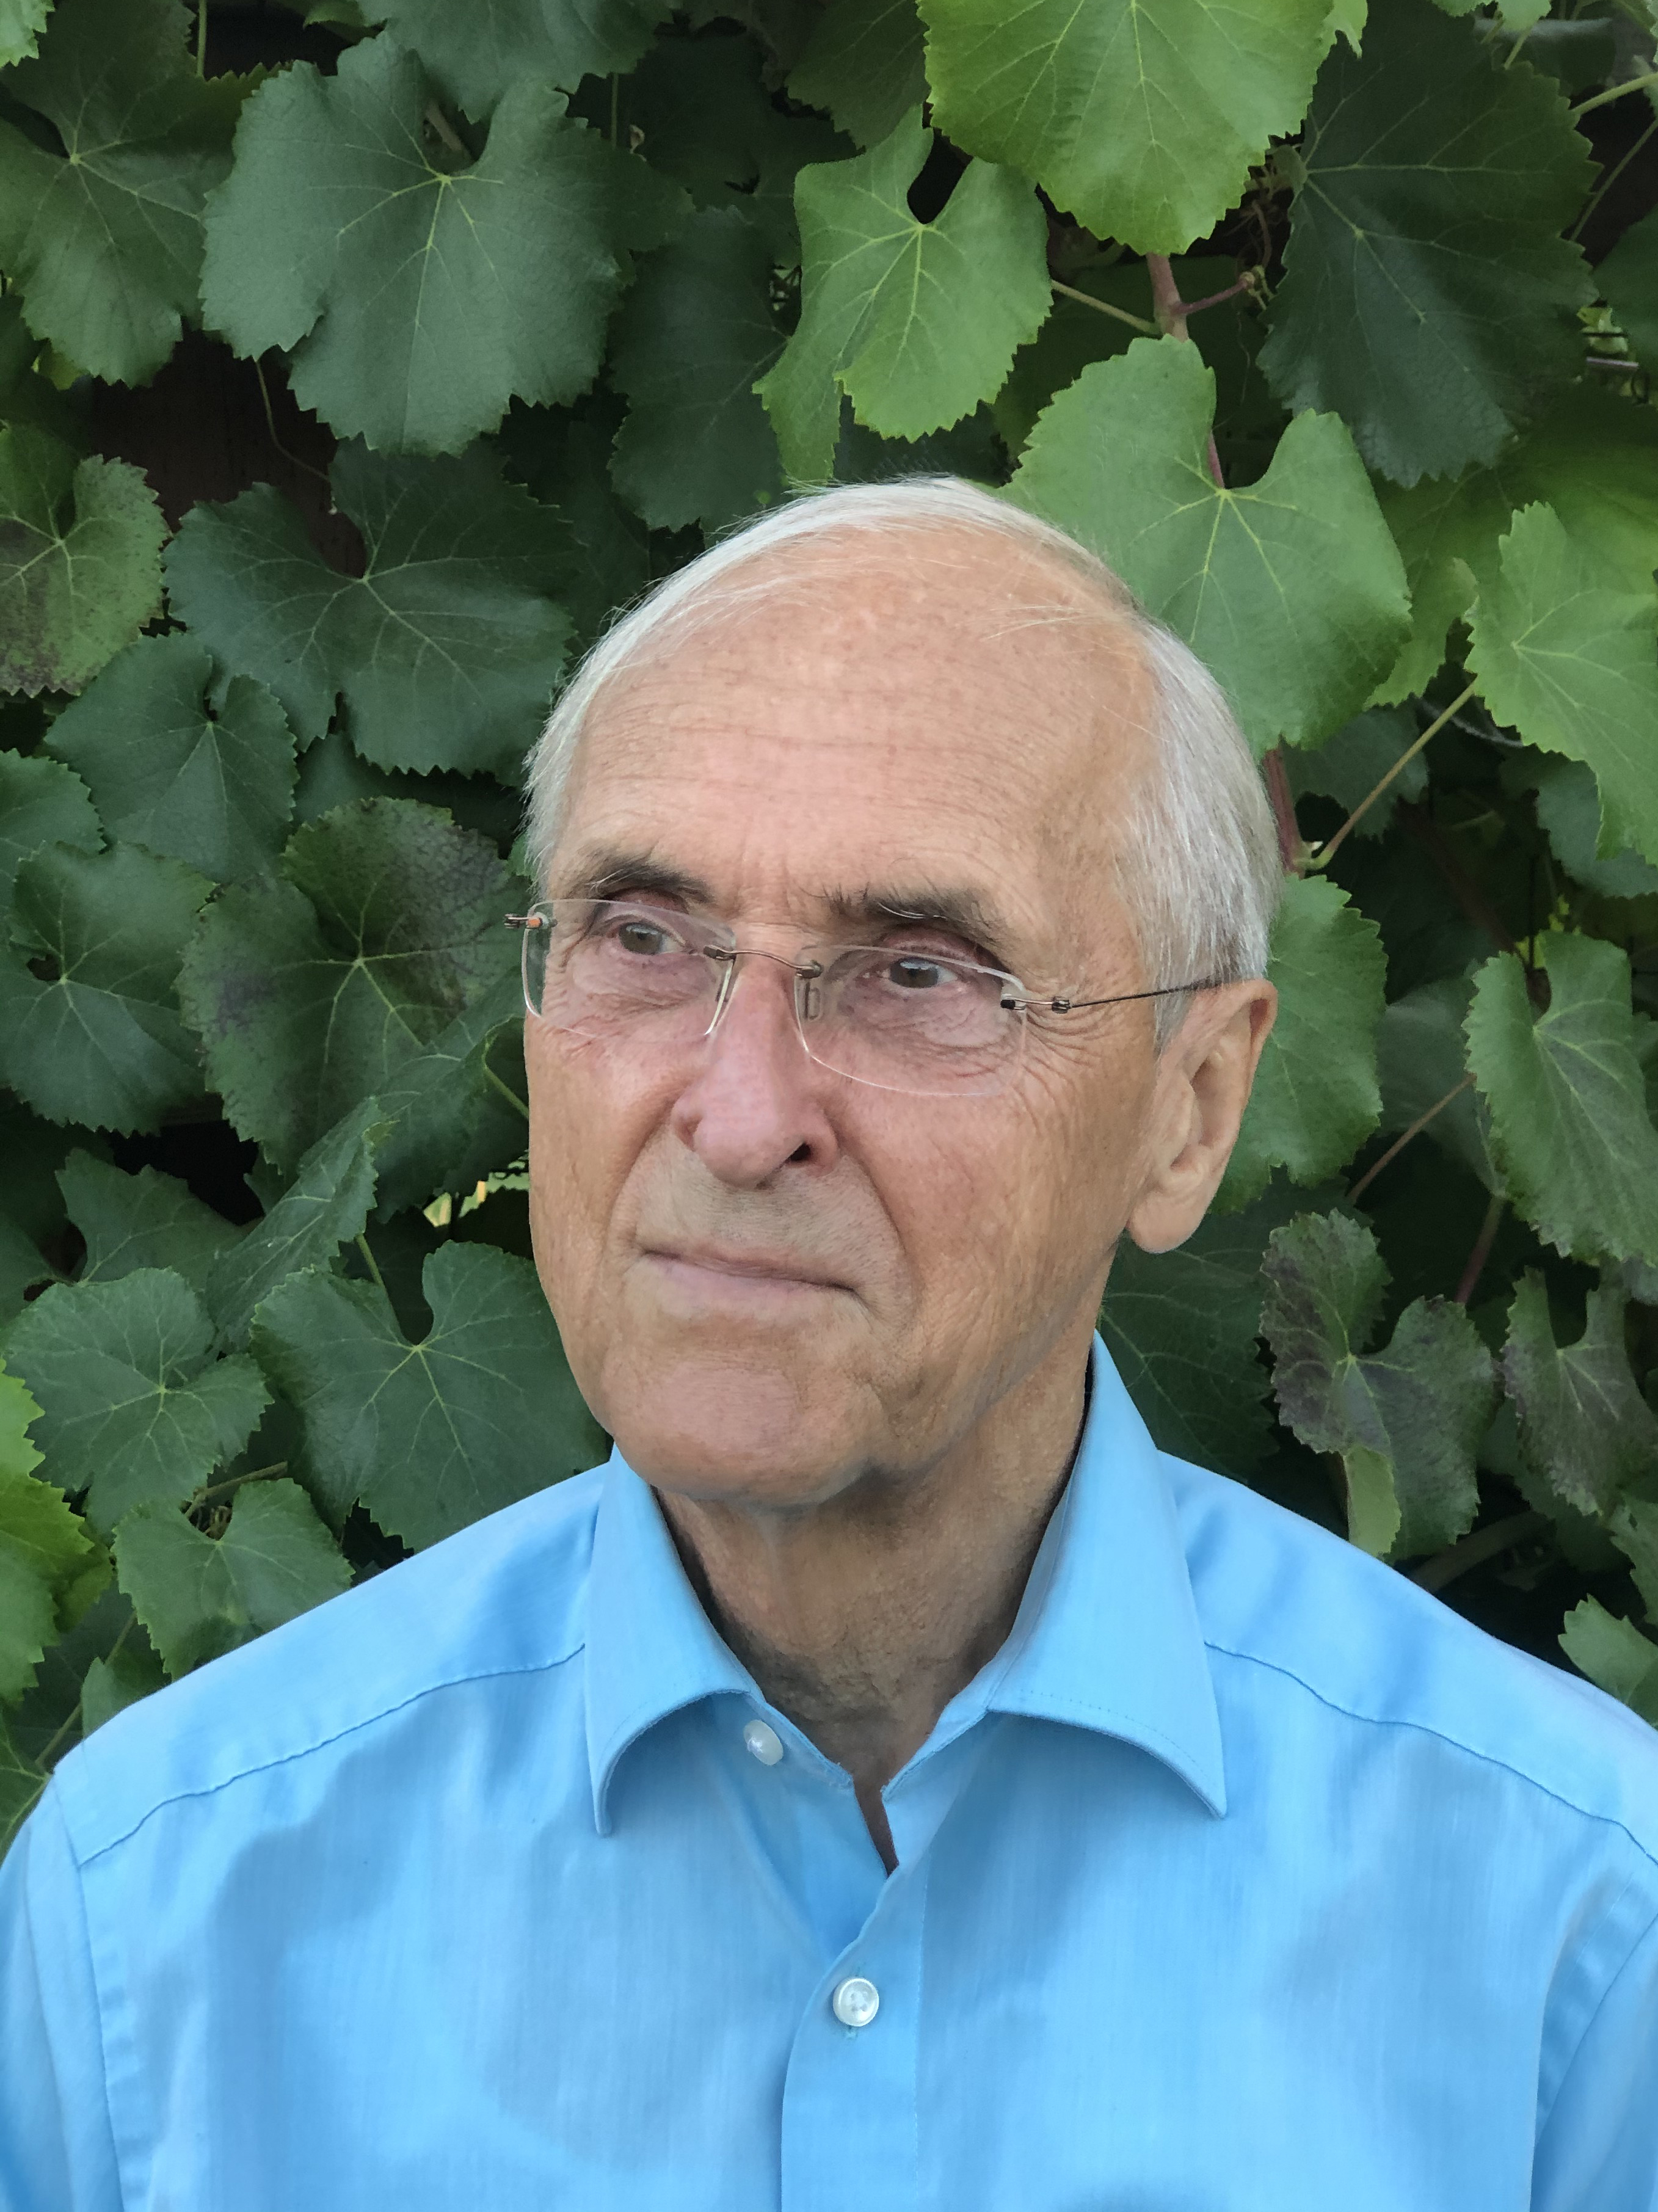
\includegraphics[width=.9\textwidth]{figures/kiparsky.jpg}
  \caption{Paul Kiparsky}
  \label{fig:ch.spe.kiparsky}
\end{wrapfigure}
The objections posed by \textsl{\isi{SPE}} to its own program as motivating
the theory of \isi{markedness} were not the only ones raised in 1968. In the
same year, an important paper by \name{Paul}{Kiparsky} asked the question `How
Abstract is Phonology?' in response precisely to the body of analyses
represented by \textsl{\isi{SPE}} and other generative work of the
1960s. The paper was initially circulated only in dittoed form;
subsequently it was made available through the semi-formal channel of
the Indiana University Linguistics Club, and it was eventually
published formally as Part 1 of \citealt{kiparsky:3dimensions}. In a
short time, the issues raised by {\Kiparsky} took on central significance
in theoretical discussion of the bases of phonology.

We argued in the previous chapter that the \isi{abstractness} of the
relation between underlying and surface forms was not in fact the
primary difference between generative phonology and its predecessors;
but that does not mean that this \isi{abstractness} was not an issue. From
within the framework of generative assumptions, {\Kiparsky} identified
two major areas in which the analytic practices of the 1960s led to
counterintuitive (indeed, demonstrably incorrect) results by paths
that were not excluded by the theory. In both classes of examples, the
cause was identified by {\Kiparsky} as excessive \isi{abstractness}: the
problematic cases involved \isi{phonological representations} that were
insufficiently constrained by the nature of the surface forms to which
they correspond.

The first set of apparently too-abstract analyses involved ``the
diacritic use of phonological features'': the positing of an underlying
phonological distinction which is never realized as such, but rather
serves to differentiate two classes of forms with respect to their
behavior under some other rule. If we were to represent the final [f]
of \textit{leaf}, which alternates with [v] in \textit{leaves}, as a
bilabial fricative [ϕ] opposed to the (non-alternating) labiodental [f]
of e.g. \textit{laugh} (/\textit{laughs}), we could then posit a
phonological rule converting [ϕ] to [v], and another rule to merge [ϕ]
and [f]. We would thus avoid any reference to the particular forms
that undergo \isi{voicing} of \emph{f} before the plural ending. The
distinction between [ϕ] and [f], however, would be purely diacritic on
this analysis: no instance of [ϕ] would ever actually surface as such,
and the difference between this segment and [f] would serve simply to
identify the class of forms that undergo \isi{voicing} as opposed to those
that do not.

The classic uses of such analyses are probably in descriptions of
\isi{vowel harmony} systems such as that of \ili{Hungarian}. In this language,
certain vowels (e.g., é [e:]) are neutral, in that they can occur
either in back-vowel words or in front-vowel words. Stems that contain
only neutral vowels usually take front-vowel variants of suffixes that
are added to them, but there is a small (closed) class of
neutral-vowel words that take back vowel suffixes: e.g., \textit{héj}
`rind, peel', \textit{ héj-am} `my rind', contrasting with
\textit{kés} `knife', \textit{kés-em} `my knife'. One possible
description of this state of affairs would be to represent words like
\textit{héj} not with underlying /é/, but rather with an otherwise
non-occurring back counterpart of this vowel: [ə:]. The \isi{vowel harmony}
rule and a (subsequent) rule converting [ə:] into [e:] could then be
stated in purely phonological terms—but the putative vowel [ə:] would
therefore never appear as such in any surface form, and the difference
between it and [e:] would serve simply to distinguish two sorts of
behavior words might show with respect to \isi{vowel harmony}.

Of course, \isi{phonological rules} must be sensitive to the phonological
composition of forms, and it may well be the case that a distinction
which conditions the differential behavior of some pair of forms with
respect to a given rule is later neutralized. For example, in \ili{English},
vowel lengthening takes place before voiced obstruents but not before
voiceless ones. In the pair \textit{rider} versus \textit{writer},
however, this distinction is later neutralized (in American \ili{English},
at least) when both /t/ and /d/ in certain environments are replaced
by flapped [D]. The difference between this analysis (which we
presumably wish to allow) and that in {\Kiparsky}'s examples is that the
latter but not the former involve \textit{absolute}
\isi{neutralization}. The difference between \ili{English} /t/ and /d/ appears in
many environments, even though it is neutralized in others, but that
between e.g. \ili{Hungarian} /e:/ and /ə:/ would never be manifested except
by its effects on other rules.

The second class of cases {\Kiparsky} suggested should be prohibited
involve ``the phonological use of diacritic features.'' By this, he
refers to analyses in which some non-phonological feature with
essentially arbitrary content is assigned to certain forms, and then
used to trigger \isi{phonological rules} which have the effect of
differentiating forms with this feature from forms without it in
surface structures. Again, \isi{vowel harmony} provides an example: some
analyses had proposed that the phonological composition of words
belonging to distinct harmony classes might be identical except for a
morpheme-sized harmony feature such as `[±B]' or the like. Thus,
\ili{Finnish} \textit{pouta} and \textit{pöytä} might both be represented as
/pOUtA/, with the former marked [+B] and the latter [$-$B]. The use of
such arbitrary features, which have no intrinsic phonetic
interpretation but serve only to trigger the operation of rules in the
grammar, would defeat the general claim that phonological
\isi{representations} should be non-arbitrary in content.

As a way of prohibiting analyses involving both of these sorts of
\isi{abstractness}, {\Kiparsky} proposed that grammars should be subject to an
\textit{\isi{alternation} condition}. It is not immediately obvious how to
formulate such a condition, but among its effects we would like to
ensure that formatives which are always the same have the same
phonological representation; and that formatives which always differ
have distinct \isi{phonological representations}. The first branch of the
condition prevents us from encoding a consistent difference of
phonological effect as a difference in phonological constituency (as
in the \ili{Hungarian} example), while the second branch prevents analyses
in which a consistent difference in phonological composition (such as
the difference between front and back vowel words in \ili{Finnish}) is
replaced systematically by some non-phonological diacritic.

{\Kiparsky} argued in favor of the correctness of some form of such a
condition on the basis of the fact that a substantial class of the
analyses which it excludes can be shown to be incorrect on independent
grounds (principally, through the use of evidence from historical
change). His points are clearly serious and cogent, and his proposed
limitation on the power of analyses was widely (though not
universally) accepted. The issue of just how strong such a condition
should be, and how it should be formulated, became a prominent topic
of discussion for the next several years. One school of thought
attempted to defend abstract analyses that constituted at least prima
facie counterexamples to the \isi{alternation condition} (including
\citet{hyman70:concreteness} for Nupe; \citet{brame72:maltese} for
Maltese; and \citet{vago73:abstract.vh} for \ili{Hungarian} and other vowel
harmony systems). Another group of linguists, however, took the
opposite tack, maintaining that the excesses of \isi{abstractness} of
\textsl{\isi{SPE}} were much more pervasive than could be dealt with by a
limited prohibition such as the \isi{alternation condition}. We deal briefly
with one set of these proposals in the next section.

{\Kiparsky}'s own attention centered on the correct delimitation of the
original set of problems, and the formulation of a condition that
would correctly exclude just these analyses. His subsequent treatment
of the problem (`Abstractness, Opacity and Global Rules', part 2 of
\citealt{kiparsky:3dimensions}) is interesting in the present context
because it is directed toward some sort of balance between
formulations involving rules and those involving \isi{representations}. He
notes that his original discussion was couched in terms of preventing
certain sorts of \isi{representations}: those in which an underlying
distinction is always neutralized, or those in which some consistent
phonological distinction is not represented phonologically. This might
be stated as a constraint on the operation of rules: `Neutralization
rules cannot apply to all occurrences of a morpheme.'

This condition by itself would not exclude all of the illicit
instances of \isi{absolute neutralization}, however. In the example of
\ili{English} alternating and non-alternating /f/, for instance, the rule
neutralizing /ϕ/ and /f/ would not apply to all instances of the
form \textit{leaf}, since in some cases /ϕ/ would be replaced by /v/ and
thus escape conversion to /f/. The analysis would thus (incorrectly)
be allowed. An alternative proposed formulation would require that
`\isi{neutralization} processes only apply to derived forms,' where
`derived' means that some aspect of the environment which permits the
application of a rule must come from a context external to any one
single formative, or else from the prior operation of some other
rule. Such a condition would exclude the analysis of leaf as /lijϕ/.

Our interest here is not in the precise formulation of the \isi{alternation}
condition. What is most important historically is simply that
phonology came quickly to realize that a purely formal theory such as
that of \textsl{\isi{SPE}} was incapable of excluding in principle a large class of
apparently incorrect analyses; and to this extent, such a theory was
intrinsically deficient as a complete representation of the nature of
\isi{sound structure} in natural language. Some additional conditions, at a
minimum, had to be imposed on the theory in order to achieve adequacy
in this domain. As a reflection of the fact that generative phonology
at this time was based on a conception of \isi{sound structure} as involving
both \isi{representations} and rules, the correct formulation of such a
condition might well involve either aspect of the grammar, or some
complex interplay between them.

\section{Constraining representations: `Natural Generative Phonology'}
\label{sec:ngp}

For some, the recognition that \textsl{\isi{SPE}} analyses could involve
unrealistically abstract relations between underlying and surface
forms was not carried nearly far enough by {\Kiparsky} and others in the
discussion of possible \isi{alternation} conditions. One line of argument
held that \isi{phonological representations} ought to keep much closer to
surface forms than did \textsl{\isi{SPE}} and other analyses coming from
generative linguists at about the same time, such as
\posscitet{lightner:thesis} analysis of \ili{Russian},
\posscitet{schane:thesis} description of \ili{French},
\posscitet{foley65:thesis} or \posscitet{harris:thesis} treatment of
\ili{Spanish}, among many others. While the specific conditions of
structuralist phonemics (such as the requirement of biuniqueness) were
by and large discredited, the spirit of a phonological representation
which could be directly and unambiguously recovered from surface forms
was far from dead.

The most completely articulated version of this program is undoubtedly
that originally associated with \name{Theo}{Vennemann} and his students at
UCLA in the early 1970s. Interestingly enough,
\posscitet{vennemann68:thesis} dissertation consisted of a rather
abstract analysis of the phonology of \ili{German}; but he soon decided that
such descriptions were more a matter of the ingenuity of linguists
than of the reality of natural language. In a paper presented in 1971,
he initiated a program based on the principle that phonological
statements should be confined to ones that are literally true of
surface forms; and \isi{phonological representations} should be regarded as
largely identical with phonetic forms.

\begin{wrapfigure}[13]{l}{.35\textwidth}
  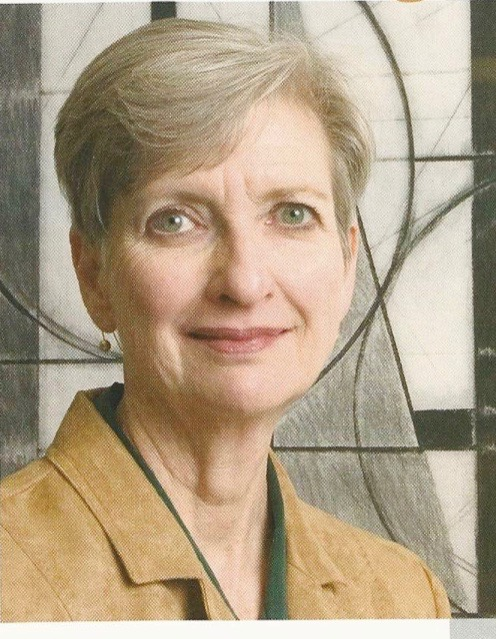
\includegraphics[width=.8\textwidth]{figures/Joan_Bybee.jpg}
  \caption{Joan Bybee [Hooper]}
  \label{fig:ch.spe.bybee}
\end{wrapfigure}
Vennemann's student \name{Joan}{Bybee} [Hooper] was largely responsible for
the subsequent elaboration and presentation of this theoretical
position to a wider audience; \citealt{hooper:ngp} remains the most
extensive statement of the theory of `Natural Generative
Phonology'. Its central notion is a proposed \textit{True
  Generalization Condition}, which requires that ``speakers construct
only generalizations that are surface-true and transparent.'' Such a
condition may sound conservative enough, but it has profound
consequences for the class of analyses allowed. In particular, it
denies the reality of \isi{phonological rules} that have even a single
exception; rules which necessarily apply prior to the operation of
some other rule which alters their environment; etc. For instance, the
rule of vowel lengthening in \ili{English} cannot be stated as a
phonological rule (or `P-Rule') in this theory, since a rule of
flapping may neutralize the difference between underlying /t/ and
/d/. Forms like [ra:jDɚ] (\textit{rider}) versus [rajDɚ]
(\textit{writer}) show that vowel lengthening is not surface-true and
transparent, and so it cannot be a phonological rule of the language.

In this and many other examples, the result is that phonological
relations must be encoded simply as more or less systematic
connections between fully-specified lexical entries. Both [rajt]
(\textit{write}) and [ra:jd] (\textit{ride}) are entered in the
lexicon as such; and the `rule' of vowel lengthening is reduced to the
status of a lexical \isi{redundancy} rule. Indeed, while details of the
nature of lexical relations within the theory vary from one
presentation to another, \isi{Natural Generative Phonology} quite typically
maintained that lexical entries are always essentially identical with
some occurring surface form. This position, then, is an instance of
the `\isi{fully specified surface variant}' theory of phonological
\isi{representations} discussed in chapter~\ref{ch.saussure_sound} above,
with the exception that in some presentations (e.g.,
\citealt{hooper75:archisegment}) a certain amount of completely
predictable detail is absent from \isi{underlying representation}s.

The great bulk of the descriptive burden on this view is borne by
conditions of well-formedness imposed on \isi{lexical representations}; but
even these can only be stated to the extent they are completely
exception-less and `surface-true'. Some \isi{systematic relations} between
forms may be stated in the form of P-Rules, insofar as they are
phonologically exception-less. Other relations between forms may be
stated as `MP' (morphophonemic) rules insofar as they have an
exception-less (and surface-true) character in terms of morphological
categories. Regularities that are not exception-less in either
phonological or morphological terms (such as the \ili{English} vowel shift
or velar softening rules) are to be considered unproductive, somewhat
anecdotal relations between individual autonomous lexical items (on a
par with {\Baudouin}'s class of traditional, paleophonetic alternations;
see chapter~\ref{ch.kazan} above). These are described (if at all) by
means of `via-rules'.

The program of \isi{Natural Generative Phonology} is one sort of reaction to
the perceived inadequacies of the account of phonetic substance
offered by \textsl{\isi{SPE}}. It attempts to remedy the presumed paradoxes
resulting from \textsl{\isi{SPE}}'s disregard of these issues by radically
restricting the conceptual richness of the theory. As such, it
represents a reaction quite analogous in character to that of
intuitionist mathematicians to the program of \textsl{PM}. Notably,
the approach of \isi{Natural Generative Phonology} required the
reconstruction of phonological accounts so as to make no appeal to
abstract entities or to (putatively) counter-intuitive logistic
principles such as that of relevant explicit ordering of rules. This
constitutes a major retreat from the idealism of \textsl{\isi{SPE}}, to a
theory founded insofar as possible on what are (from the point of view
of a linguist, if not that of an experimental psychologist) the
observable and immediately verifiable aspects of linguistic
structure. As such, it is immediately reminiscent of the
constructivist basis of intuitionist \isi{mathematics}.

In fact, the parallel is quite close. \isi{Natural Generative Phonology}
succeeded in reconstructing a substantial part of the traditional
domain of phonological description, though sometimes in rather
unfamiliar terms. In doing so, it showed much about the conceptual
basis of more familiar accounts. On the other hand, there are also
many aspects of what has usually been taken to be phonology which are
inaccessible on its premises. These areas of phonology are either
written off altogether (that is, declared to be linguistically
meaningless) or ascribed to the operation of essentially non-linguistic
or unsystematic principles (such as the `via-rules', essentially a
name for the description of those aspects of phonology that cannot be
accounted for without recourse to abstract entities).

A program of this sort is effectively impossible to falsify, since it
consists not in a potentially verifiable claim about the object of
linguistic study but in an externally imposed limitation on the object
of such study. It is always possible, of course, to confine one's
attention to certain types of fact to the exclusion of others; and to
accord the name `linguistics' only to what can be studied in this
way. This procedure, however, should not be confused with a genuinely
empirical result about the nature of language, which can only come
from the effort to construct substantive explanatory theories for
domains whose exact delimitation follows from the scope of the
principles that they reveal, rather than being given completely in
advance.

Now a consistent advocate of the `Natural Generative' theory may well
be happy with the result that certain domains are legislated out of
consideration, just as a confirmed intuitionist may be convinced of
the result that much of classical and modern \isi{mathematics} is literally
meaningless. In both areas, though, the majority of traditional,
pre-systematic practitioners have felt discontent with the limited
portions of their field that can be treated within such radically
constructivist accounts. A number of detailed examinations of Natural
Generative Phonological analyses (such as those of
\citet{harris78:morphophonology} and \citet{gussmann:abstract})
concluded that the theory had the result of throwing out the baby with
the bath water. By the mid-1980s, the great majority of phonologists
had in general concluded that whatever \textit{a priori}
considerations of `psychological reality' may motivate it, this way of
avoiding the disregard of phonetic substance characteristic of
\textsl{\isi{SPE}} was unsatisfactory as a basis for understanding the sound
structures of natural languages.

It should be noted that, although advocates of Natural Generative
Phonology consistently portrayed their position as a theory quite
distinct from that of generative phonology, a single overall set of
underlying assumptions about what sorts of thing constitute evidence
and valid modes of inference about theoretical issues is largely
common to `natural' and `orthodox' (or `standard theory') generative
phonologists. From this, we can conclude that Natural Generative
Phonology constituted an attempt to reform the theory from within,
rather than a fundamentally different theory (in the way generative
phonology surely constituted a different theory from that of American
structuralists in the late 1950s and early 1960s). This does not
of course trivialize the enterprise; but it does mean that `natural'
and `orthodox' generative analyses are not as incommensurate with each
other as both sides sometimes asserted.

This fact is essential to an understanding of the ultimate impact of
\isi{Natural Generative Phonology}. The radical restrictions on phonological
analyses proposed in this theory found few advocates, though it is
hard to deny that a gradual trend toward more concrete accounts of
phonological systems and a reduced reliance on highly abstract
mechanisms among generative phonologists in the late 1970s and early
1980s resulted in part from the challenges Natural Generative
Phonology mounted to the unrestrained use of the descriptive power of
the \textsl{\isi{SPE}} theory. The principal effect was on the
prevailing conception of \isi{phonological representations}, as is only
natural given the rather impoverished notion of \isi{phonological rules}
that Natural Generative phonologists maintained.

Although there was little explicit, overt agreement on this point in
the literature, the descriptive practice of the field was considerably
altered in a more conservative direction as a direct consequence of
the arguments of \isi{Natural Generative Phonology}. An example is the
effect on analyses of \ili{French} such as that of
\citet{tranel81:french}. This effect resulted quite directly from the
fact that, at bottom, the positions involved share the majority of
fundamental assumptions about how linguistic inquiry is conducted,
what constitutes evidence, etc. The specific \textit{a priori}
limitations on the field proposed by Natural Generative phonologists
were widely (though not universally) judged to have been misguided,
but insofar as specific analyses constructed along these lines could
be supported by concrete evidence, they could be directly incorporated
into other sets of views.

\section{Constraining rules: Natural Phonology}

The major thrust of the reaction against the \textsl{\isi{SPE}} theory in
the 1970s was grounded in the sense that although such a theory might
(if appropriately modified, along lines such as those suggested by
{\Kiparsky}) capture what is possible in the sound systems of natural
languages, it was intrinsically incapable of representing what is
natural about such systems. The very name `Natural Generative
Phonology' was of course intended to imply that any other sort of
generative phonology was not `natural'. Other theoretical positions
which developed during this period (e.g., the present author's theory
of `natural ordering' in \citealt{sra74:orgphon}) similarly attempted
to trade on the favorable connotations of the word `natural'. Among
these works purporting to refound phonological thought on bases closer
to those of the organic sources of language, surely the most
interesting (and most explicit in this regard) is the theory of
`\isi{Natural Phonology}' developed by \name{David}{Stampe} and his colleague
\name{Patricia}{Donegan}, as originally presented in works such as
\citealt{stampe68:yes.virginia,stampe69:acquisition}, and most
comprehensively in \citealt{stampe:thesis} and
\citealt{donegan.stampe79:study.of.np}.\footnote{\citet{donegan.stampe09:hypotheses}
  provide a recent updated account of the principles of the theory,
  highlighting among other things associations of the scope of
  particular processes with prosodic categories.}

{\Stampe}'s critique starts from a consideration of the same puzzles for
a purely formal theory that motivated the theory of \isi{markedness} in
\textsl{\isi{SPE}}: some phonological systems and rules are much more likely
to occur in languages than others, and this must somehow be part of
the essence of language which it is the business of the theory to
capture. Unlike the \isi{markedness} theory of \textsl{\isi{SPE}}, however, he
rejects the attempt to encode these facts about what is and is not
natural in the notation \citep{stampe73:chap9}. Rather, he recognizes
that natural rules, as well as effects of the \isi{constraints} imposed on
phonological systems by the nature of language, are nonetheless
aspects of the grammars of particular languages. The insight
underlying his view is that there are some rules and \isi{constraints} which
are more expensive for a language \textit{not} to have; that is,
languages which are not subject to them are in some sense more complex
than languages that are. Much of the theory of \isi{Natural Phonology} is
devoted to an attempt to articulate the sense in which this is true.

The basis of the theory is the claim that our innate phonetic capacity
can be represented in the form of a set of very general
\textit{natural processes}. These can be classified into two groups:
\textit{syntagmatic processes} (later reformulated as
\emph{lenitions}), which reduce the complexity of articulating
particular (segments or) sequences of segments (as with rules
assimilating nasals to following obstruents, or \isi{nasalizing} vowels
before \isi{nasal consonants}); and \textit{paradigmatic processes} (later,
\emph{fortitions}), which highlight or maximize the articulatory or
perceptual properties of a segment or sequence (such as a rule
specifying that vowels are generally [$-$nasal], given that nasal
vowels are less distinct from one another perceptually than are
non-\isi{nasal vowels}). As is evident, these two classes may make
contradictory demands on a given segment: a vowel preceding a nasal
consonant should be [$-$nasal] by virtue of the paradigmatic process
of denasalization, but [+nasal] by virtue of the syntagmatic process
assimilating nasality. Such conflicts are resolved either by general
principle (``fortitions precede lenitions'') or as a matter of
language-particular limitation of one or the other process.

The inventory of natural processes is assumed to constitute part of
the genetically determined endowment which the language learner brings
to the task of acquisition. In fact, on this view, the essential
nature of that task is precisely that of learning to suppress and
limit those natural processes which are not fully general in the
language to be learned. Thus, a \ili{French} (but not an \ili{English}) child must
learn to limit severely the domain of application of vowel
denasalization, since \isi{nasal vowels} appear in that language. The kinds
of limitation involved may involve not only complete suppression of a
process, or restriction of the range of cases to which it applies, but
also the imposition of an ordering relation on it, such that its
applicability is limited to forms to which some other process has not
yet applied.

\begin{wrapfigure}[12]{l}{.35\textwidth}
  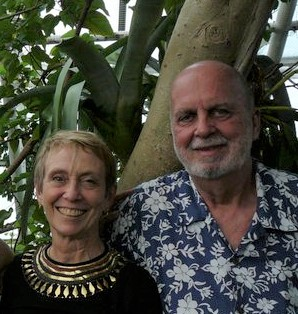
\includegraphics[width=.9\textwidth]{figures/Donegan-Stampe.jpg}
  \caption{Patricia Donegan and David Stampe}
  \label{fig:ch.spe.donegan-stampe}
\end{wrapfigure}
In addition to natural processes, languages are also assumed to
contain learned \textit{Rules}—but these are taken to be rather
limited, \textit{ad hoc} and unsystematic \isi{constraints}, generally tied
to morphological categories, descriptive of alternations that are
consequences of the accidental history of the language (comparable to
the \isi{arbitrariness} of the fact that, in \ili{English}, the word \textit{dog}
designates dogs). As such, they are said to fall outside of the
explanatory domain of phonology proper, and into the realm of the
purely conventional. \isi{Natural Phonology} thus attempts to provide an
account of ``everything that language owes to the fact that it is
spoken'' \citep[128]{donegan.stampe79:study.of.np}, and to ``exclude
the topic of unmotivated and morphologically motivated alternations''
(\textit{Ibid}., p. 127) such as \ili{German} Umlaut or \ili{English} velar
softening.

In the data of natural languages, phonological patterns naturally do
not wear on their sleeves an indicator of the group (natural processes
or learned rules) from which they derive. It is thus necessary to
establish from the outset what qualifies a given \isi{alternation} for the
status of a natural process, since it is only these that the theory
has anything to say about. In this regard, the central point is that
natural processes appear ``unbidden and unlearned'': i.e., positive
evidence is not necessary for them to arise, but only the lack of
negative evidence. They thus show up in the substitutions children
make in the forms of adult language, in rules of casual or fast
speech, in \isi{historical change}—as well, of course, as in rules of adult
grammars (where, however, they coexist with learned rules).

The great attractiveness of this theory is quite similar to that of
\posscitet{jakobson:kindersprache} \textsl{Kindersprache} (see
chapter~\ref{ch.jakobson} above): both promise to unify large domains
of phenomena that fall outside the strict notion of the `grammar' of a
language but are nonetheless clearly related to the nature of
language. This similarity is of course not accidental, since {\Stampe}
explicitly modeled his program on {\Jakobson}'s. Such a theory makes very
strong claims about the nature of language, and these claims are
immediately open to a wide range of potential confirming or
discontinuing evidence (assuming they are not simply metaphorical).

\citet{dressler74:puzzles} examined some of the claims of natural
phonology in the domain of \isi{historical change}, and pointed out a number
of difficulties. He cites, for instance, a number of (context-free, or
paradigmatic) historical changes of the form [u] > [ü], in which no
intermediate stages can be motivated. Such changes have taken place in
the history of \ili{French}, \ili{Icelandic}, and other languages. The importance
of this fact (and a number of comparable ones cited by Dressler\ia{Dressler, Wolfgang U.}) is
that it is directly contrary to a presumed hierarchy of \isi{naturalness}
governing vowel systems, according to which front rounded vowels
should be replaced either by back rounded or by front unrounded
vowels, but not vice versa. In order to incorporate such examples, it
is necessary to assume that `natural processes' are in some sense
two-way streets along which substitutions can occur. If true, this
would greatly weaken the empirical content of the theory.

One of the most extended analyses of the claims made by the theory of
natural phonology was provided by \citet{drachmann:kindersprache} in
the context of an examination of putative similarities between child
and adult language substitutions. Among Drachmann\ia{Drachmann, Gaberell}'s points are the
following: (1) children tend to substitute \isi{stops} for \isi{fricatives},
through the replacement of a gesture of continuous control by a
ballistic one—but in adult language such changes are much less common
than the reverse process of spirantization of \isi{stops}. (2) Children
typically shorten words by removing their initial \isi{syllable}(s). The
fact that it is final syllables that are retained can be seen as due
to a `recency' effect; but in adult language, \isi{phonological rules} and
\isi{historical change} operate almost exclusively to reduce or eliminate
\textit{final} syllables. (3) In \isi{child language} acquisition, the very
general processes of `\isi{vowel harmony}' seem to be suppressed early,
while comparable consonantal assimilations across a word persist much
longer. In adult language, however, \isi{vowel harmony} is comparatively
common, while consonant harmony (especially on the scale observable in
\isi{child language}) is rare or nonexistent.

These points seriously compromise the underlying assumptions of
\isi{Natural Phonology}, for they suggest that the coherence of the theory
is not matched by the facts. The claim that what is natural in the
systems of adult languages has its basis in whatever more general
aspects of our phonetic capacities operate in other domains (such as
\isi{child language}, casual speech simplifications, \isi{historical change},
etc.) can only be substantiated by a demonstration that these domains
are in fact homologous—and a detailed examination of the evidence
suggests that the similarities that do exist are too limited to
sustain the weight of a comprehensive theory of phonological
\isi{naturalness}.

If we attempt to limit the explanatory domain of phonology to the set
of natural processes in {\Stampe}'s sense, the result is that any
\isi{alternation} which is not phonetically motivated, or shows phonetically
arbitrary properties, immediately falls into the category of learned
rules and thus outside of the theory. In that case, however, a great
deal of the descriptive content of the sound systems of natural
languages—perhaps, indeed, nearly all of it—is not describable as
`phonology' in this sense at all.

As observed already by {\DeCourtenay} (chapter~\ref{ch.kazan}),
even those processes with the most evident phonetic motivation tend to
acquire arbitrary aspects once they become part of the grammar of a
particular language (`phonologized'). A number of examples of this
sort are examined in \citealt{sra81:unnatural}; these will not be
repeated in detail here.\footnote{Both
  \citet{dressler84:explaining.np} and
  \citet{donegan.stampe09:hypotheses} complain that
  \citet{sra81:unnatural} attacks a ``straw man'' in this paper. Since
  neither paper explains the basis of this objection, or engages directly
  with the examples discussed, it is difficult to provide an effective
  reply.} The thrust of the argument is not at all that the phenomena
treated in the \isi{Natural Phonology} literature are uninteresting or
inappropriately characterized. The claim that articulatorily and
perceptually grounded processes drive the ``categorical discrepancies
between speech as it is perceived and intended, and speech as it is
targeted for actuation'' \citep[1]{donegan.stampe09:hypotheses} is a
plausible and appealing one, and the explanatory domain of the
principles invoked is substantial. The point is, rather, that this
domain does not at all exhaust the study of sound patterns in
language.

Any phonologist who has worked out the system of a language in detail
will be aware that while much of its sound pattern does indeed find
its grounds in the operation and interaction of natural processes of
the sort studied by {\Stampe} and {\Donegan}, there is much else
besides. Even apparently low-level, automatic phonetic processes such
as vowel lengthening before voiced obstruents in \ili{English} may have
aspects that are not reducible to the operation or scope of
universally available natural processes or their interaction with one
another: in this case, studies have long shown that the degree of
lengthening observed in \ili{English} is not phonetically explicable, but
must be regarded as an arbitrary fact about the language. To the
extent this is the case, the \isi{regularities} observed must be relegated
to the domain of ``rules'' and not ``processes'', and thus excluded
from the scope of phonology as this is characterized in Natural
Phonology. 

A similar example is provided by the fronting of velars to palatals
before front vowels in \ili{Icelandic}
\citep[100ff.]{arnason11:icel.far.phonology}. Such an accommodation of
articulatory place occurs more or less automatically in most of the
world's languages, and is surely a candidate for the status of a
natural process, but in \ili{Icelandic} applies before some vowels that are
no longer phonetically front ([ai̯], the modern reflex of earlier [æ]),
although they used to be, and not before others that are front but
that come historically from back vowels ([ü] and [ö], historically [u]
and [ɔ]). Again, the accretion of phonetically unmotivated
complications (the result of diachronic change, in this instance)
would consign the otherwise quite natural rule of velar \isi{palatalization}
in \ili{Icelandic} to the category of a rule outside the scope of
phonology.\footnote{\citet[48]{dressler84:explaining.np} cites this as
  an instance of ``confusions of rules and processes in the
  literature.'' On the contrary, it was cited as an example in which
  language-particular eccentricities force its classification as a
  rule, not a process, and thus outside the scope of phonology in the
  NP sense, despite its manifestly well motivated core and origins.}

Apparently, then, if we exclude all facts from phonological
consideration that show a component of purely language-particular
\isi{arbitrariness}, much less will remain than might be expected. If we
furthermore require that the natural processes which constitute the
empirical content of the theory operate in a more or less uniform
fashion across several domains (\isi{child language}, etc., as well as the
rules of adult language), even less will be left to us. For this
reason, the theory of \isi{Natural Phonology} remained at the level of a
suggestive hypothesis, though it is one which has been applied to a
substantial range of empirical phenomena (especially in the work of
{\Stampe} and {\Donegan}; see for example \citealt{donegan78:vowels} and
references in \citealt{donegan.stampe09:hypotheses}). It should be
noted that there are important themes common to \isi{Natural Phonology} and
\isi{Optimality Theory}, a matter that will be noted in
section~\ref{sec:rise-ot} in the following chapter.

There is clearly something general and natural about phonological
systems which is not represented in a system of the \textsl{\isi{SPE}} type;
and it is plausible to seek explanations of that fact in the organic
basis of human phonetic capacities. Where the theory of \isi{markedness} in
\textsl{\isi{SPE}} and that of \isi{Natural Phonology} went astray (in different
ways), I suggest, was in trying to incorporate this \isi{explanation}
directly into the very notion of phonology, building \isi{naturalness}
considerations into the notation characterizing all phonological
effects, however arbitrary, in the first case, and in the second,
confining the scope of phonology to those effects for which such an
account is (exhaustively) available. We should instead recognize the
modularity of language: the fact that it represents the intersection
of a number of distinguishable domains, each subject to its own
principles.

In these terms, it can be suggested, a fundamentally modular theory
with a serious claim to genuine explanatory capacity already existed
\textit{in posse} in the views of {\Baudouin} and {\Kruszewski} sketched in
chapter~\ref{ch.kazan}. On that picture, the phonetic capacities of
speakers function to determine the `raw material' for \isi{sound change} and
other substitutions, which serve as the source of synchronic
\isi{regularities} in natural language systems. The impact of such `natural
processes' on phonological systems, however, is a result both of their
substantive content and of the interaction of this with the processes
of \isi{phonologization} and \isi{historical change} \citep{sra16:explanations} —
for once incorporated into the cognitive system of a language, they are no
longer phonetically determined in their essence. Many (if not most) of
the details of such a theory remain to be developed, but at least in
outline it appears to present the possibility of achieving an
understanding of the scope of `phonetic \isi{explanation}' in phonology,
without abandoning the requirements of comprehensive and accurate
description.

Though we have suggested above that the theory of \isi{Natural Phonology}
went too far in combining the projects of description and \isi{explanation} in
phonology, its impact on the field was not at all negligible. If
phonologists from the 1970s on became increasingly aware of the need to
supplement purely formal theories with an account of substantive
considerations, this was not at all exclusively as a result of the
theory of \isi{markedness} in \textsl{\isi{SPE}}. A suggestive case was made
there, but the \isi{mechanism} proposed seems to have been a dead end. The
rather different proposals of \isi{Natural Phonology} tended to remain
somewhat programmatic (indeed, some would say, oracular) and were not
really translated into comprehensive descriptions of actual languages;
but their much greater empirical scope (in comparison to \textsl{\isi{SPE}})
tended to keep the problems they addressed within the attention of the
field at large.

\begin{figure}
  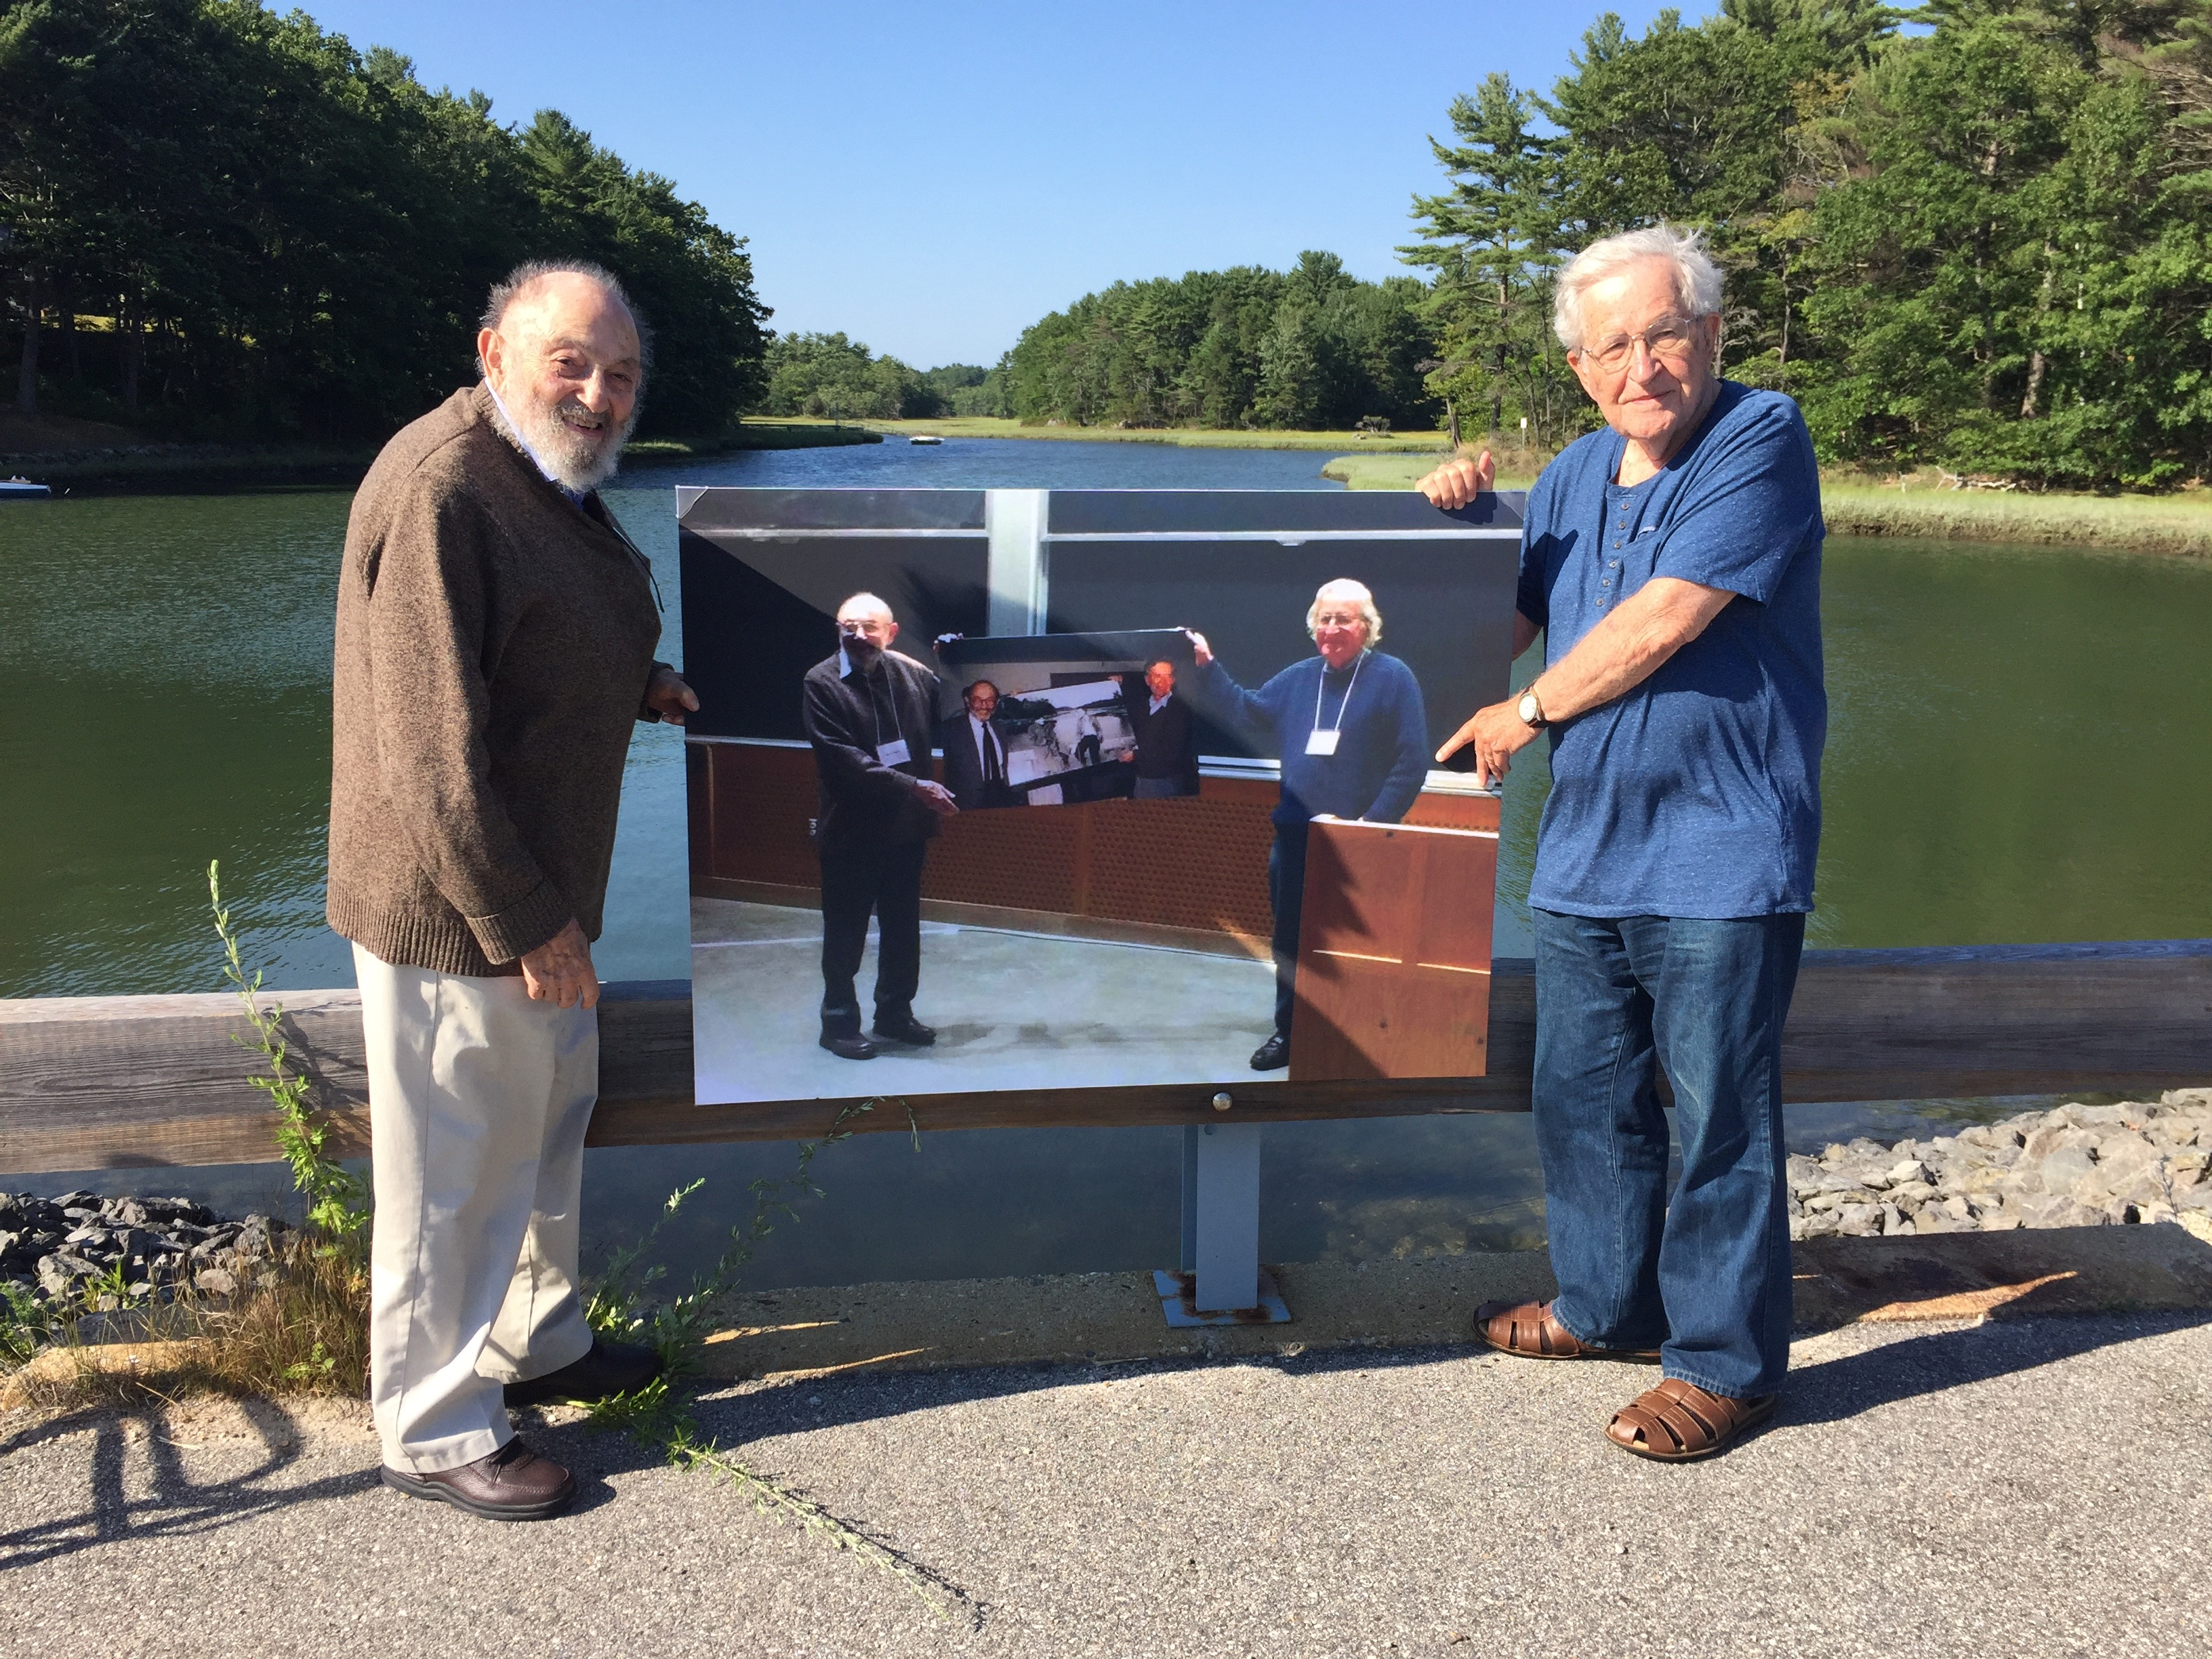
\includegraphics[width=.9\textwidth]{figures/Recursion.jpg}
  \caption{Morris Halle and Noam Chomsky over the years\\
    (2016 (2011 (1988 (1955))))}
  \label{fig:ch.spe:hallechomsky}
\end{figure}


%%% Local Variables: 
%%% mode: latex
%%% TeX-master: "/Users/sra/Dropbox/Docs/Books/P20C_2/LSP/main.tex"
%%% End: 
